% Ivan Hip / 2019-05-07

\documentclass{beamer}
\usetheme{Frankfurt}

% Ivan Hip / 2019-05-08
% iskustvo je pokazalo da kod korištenja Beamera treba učitati ove pakete

\usepackage[croatian]{babel}
\usepackage[utf8]{inputenc}
\usepackage[T1]{fontenc}
\usepackage{lmodern}

\hypersetup{unicode = true}

% Ivan Hip / 2019-05-08
% jedinstveni naslovni slajd za prezentacije

\newcommand{\naslov}[1]{
	\title{#1}
	\author{Ivan Hip}
	\institute{Geotehnički fakultet, Sveučilište u Zagrebu}
	\date{
\includegraphics[width=0.15\textwidth]{../CC-by-sa.pdf}}
} % \newcommand

\newcommand{\naslovnislajd}{
	\begin{frame}
		\titlepage
	\end{frame}
} % \newcommand

\naslov{Tečenje u cijevima}

\begin{document}
\naslovnislajd

\section{Uvod}
\begin{frame}{Tečenje u cijevima (engl. \emph{pipe flow})}

\begin{center}
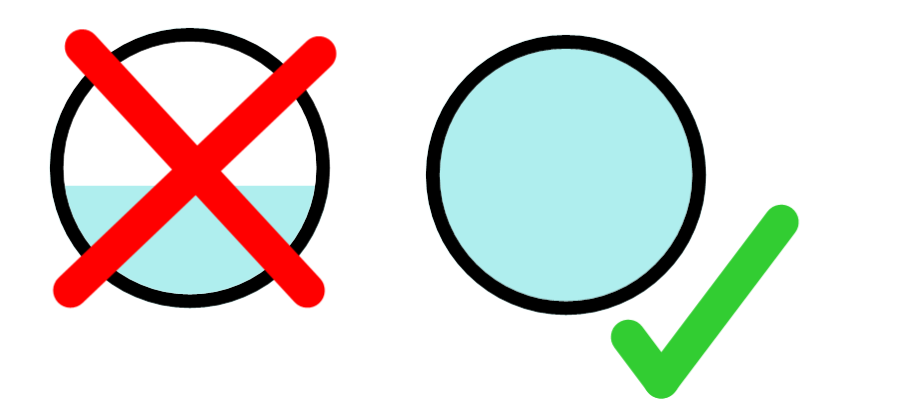
\includegraphics[width=0.5\paperwidth]{slike/slika1.PNG}
\par\end{center}
\begin{itemize}
\item kod tečenja u cijevima podrazumijevamo da je cijev u potpunosti ispunjena
tekućinom kako bi se na njenim krajevima mogla uspostaviti razlika
tlakova
\item u početku ćemo se baviti samo cijevima kružnog presjeka
\item radi jednostavnosti bavit ćemo se samo \alert{stacionarnim tečenjem}
\end{itemize}
\end{frame}

\begin{frame}{Razlika tlakova na krajevima cijevi}

\begin{center}
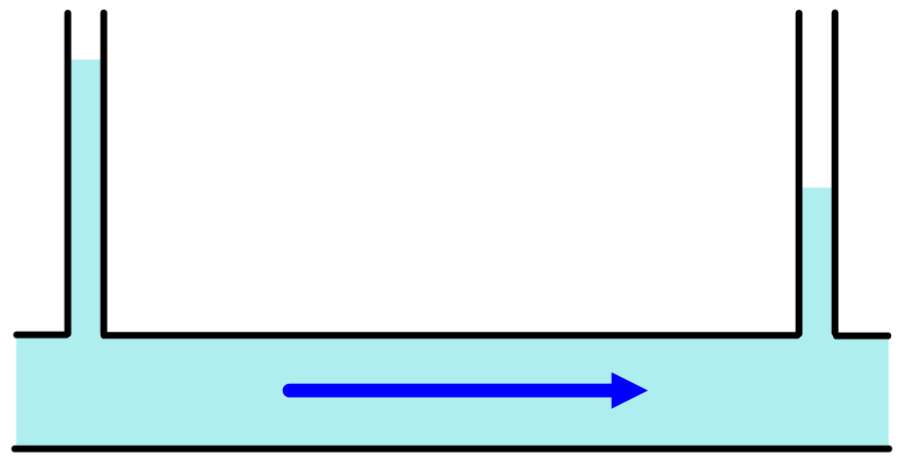
\includegraphics[width=0.5\paperwidth]{slike/slika2.PNG}
\par\end{center}
\begin{itemize}
\item za tečenje u horizontalnoj cijevi nužna je razlika tlakova na krajevima
cijevi
\item ukoliko je razlika tlakova stalna dolazi do stacionarnog tečenja,
a ukoliko je i promjer cijevi stalan tečenje je \alert{jednoliko},
tj. na svakom presjeku cijevi ista je srednja brzina tekućine $\bar{v}$
\end{itemize}
\end{frame}

\begin{frame}{Viskozno trenje}

\begin{center}
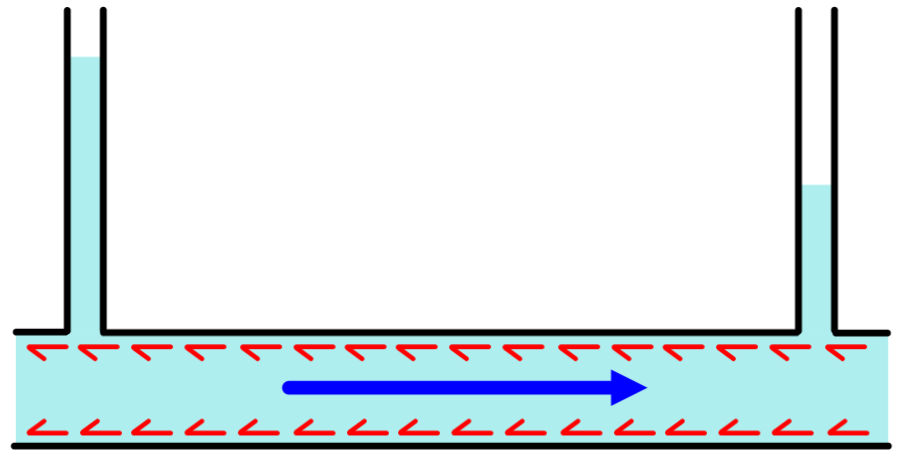
\includegraphics[width=0.5\paperwidth]{slike/slika3.PNG}
\par\end{center}
\begin{itemize}
\item pad tlačne visine ujedno znači da se smanjila specifična elastična
potencijalna energija tekućine, međutim, kako nije došlo do povećanja
brzine, jasno je da se ona nije pretvorila u kinetičku energiju, već
je na neki način izgubljena
\item kod tečenja stvarnih (realnih) tekućina nužno se javlja viskozno trenje
zbog kojeg se dio mehaničke energije tekućine pretvara u toplinu,
tj. unutarnju energiju tekućine
\end{itemize}
\end{frame}

\begin{frame}{Gubitak tlačne visine zbog viskoznog trenja}

\begin{center}
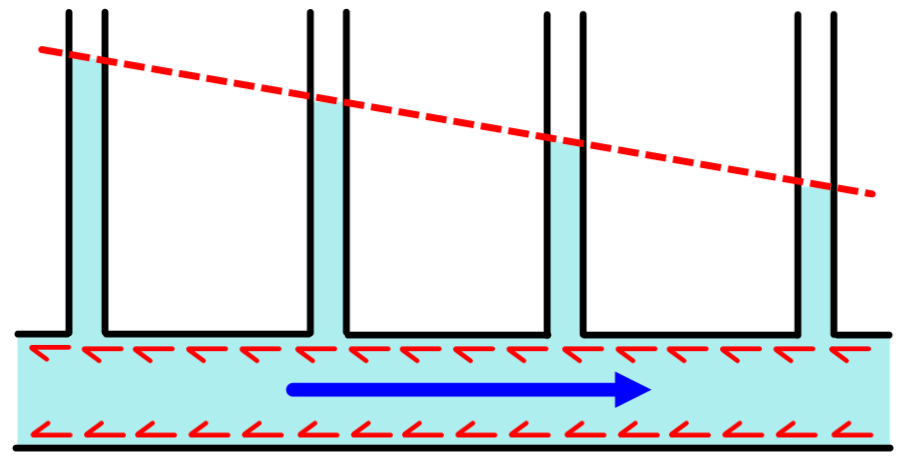
\includegraphics[width=0.5\paperwidth]{slike/slika4.PNG}
\par\end{center}
\begin{itemize}
\item kod jednolikog tečenja sila viskoznog trenja koja se opire tečenju
je istog iznosa (ali suprotne orijentacije) kao i sila koja se javlja
uslijed razlike tlakova na krajevima cijevi i uzrokuje tečenje
\item pad visine po jedinici duljine cijevi $\Delta h/L$ je kod jednolikog
tečenja konstantan, a time je i $\Delta p/L=konst.$ 
\end{itemize}
\end{frame}

\section{Laminarno tečenje kroz horizontalnu cijev}
\begin{frame}{Jednoliko tečenje u slojevima}

\begin{center}
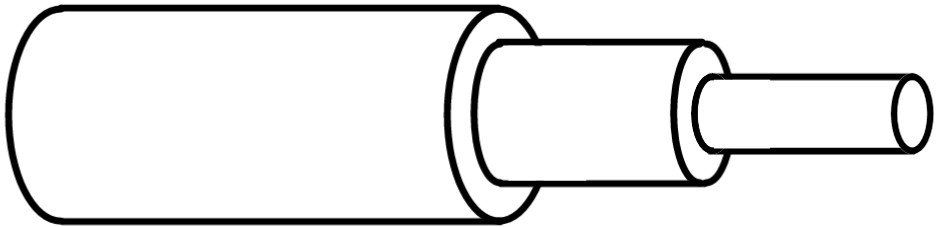
\includegraphics[width=0.5\paperwidth]{slike/slika5.PNG}
\par\end{center}
\begin{itemize}
\item zbog lijepljenja tekućine za stijenke cijevi (\emph{no-slip condition!})
logično je pretpostaviti da će brzina strujanja uz stijenke cijevi
biti manja od brzine u unutrašnjosti cijevi
\item za cijev kružnog presjeka prirodno je na presjeku koristiti polarni
koordinatni sustav s ishodištem u centru (na osi) cijevi i koordinatom
$r$ koja se kreće od $0$ (os cijevi) do ruba (stijenke) cijevi na
udaljenosti $R$ od osi ($R$ je polumjer cijevi)
\item zbog kružne simetrije razumno je pretpostaviti da će brzina ovisiti
samo o udaljenosti od osi cijevi, tj. o parametru $r$
\end{itemize}
\end{frame}

\begin{frame}{Sile na valjkasti element tekućine}

%\begin{spacing}{0}
\begin{center}
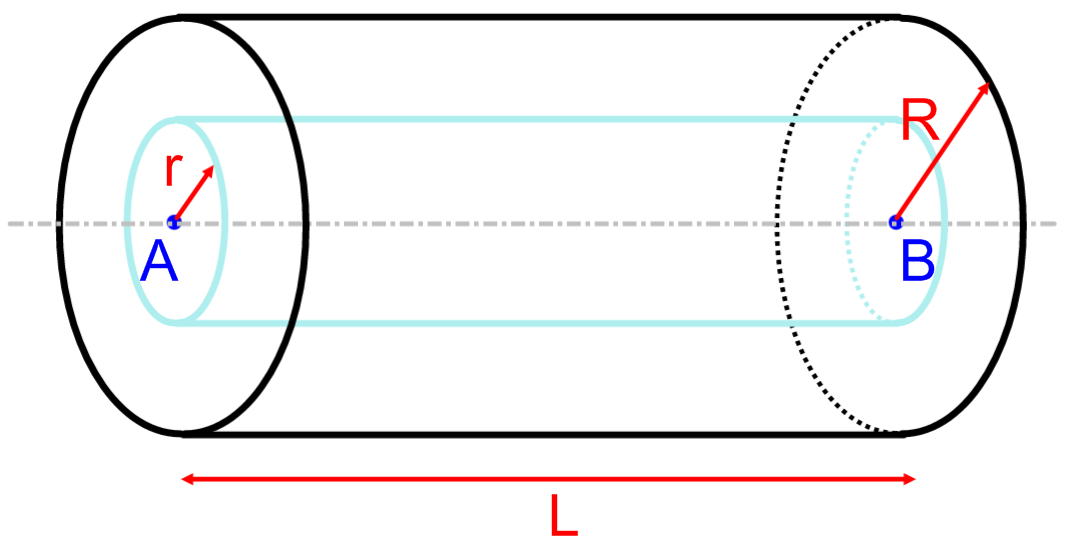
\includegraphics[width=0.5\paperwidth]{slike/slika6.PNG}
\par\end{center}
%\end{spacing}
\begin{itemize}
\item zbog razlike tlakova na bazama valjka javlja se sila iznosa
\[
F_{_{\Delta p}}=p_{_{A}}S_{_{A}}-p_{_{B}}S_{_{B}}=(p_{_{A}}-p_{_{B}})S_{baze}=\Delta p\:\pi r^{2}
\]
\item zbog viskoznog trenja javlja se posmično naprezanje $\tau$ na plaštu
valjka te je iznos ukupne sile viskoznog trenja
\[
F_{vt}=\tau\,S_{pla\check{s}ta}=\tau\:2\pi rL
\]
\end{itemize}
\end{frame}

\begin{frame}{Ovisnost posmičnog naprezanja o r}

Ako je gibanje duž cijevi jednoliko, to znači da su sile u ravnoteži
\[
\vec{F}_{_{\Delta p}}+\vec{F}_{vt}=\vec{0}
\]
to jest sile $\vec{F}_{_{\Delta p}}$ i $\vec{F}_{vt}$ su suprotno
orijentirane, ali imaju isti iznos
\[
F_{_{\Delta p}}=F_{vt}\quad\Rightarrow\quad\Delta p\,\pi r^{2}=\tau\,2\pi rL\quad\Rightarrow\quad\tau(r)=\frac{1}{2}\frac{\Delta p}{L}r
\]

Kako je omjer $\Delta p/L=konst.$ posmično naprezanje $\tau$
ovisi linearno o udaljenosti od osi cijevi: na osi je nula, a najveće
naprezanje je na stijenki cijevi kada je $r=R$
\[
\tau(r=R)=\frac{1}{2}\frac{\Delta p}{L}R
\]

\end{frame}

\begin{frame}{Veza koordinata y i r}

\begin{itemize}
\item posmično naprezanje uzrokovano viskoznim trenjem je
\[
\tau=\mu\frac{dv}{dy}
\]
\item koordinata $y$ mjeri se od kontaktne površine između tekućine i cijevi,
dakle od stijenke cijevi prema unutrašnjosti
\item mi trebamo obrnuti koordinatni sustav gdje se $r$ mjeri od osi cijevi
prema stijenki pa nam treba veza između tih koordinata
\item za svaku točku $T$ mora vrijediti $y_{_{T}}+r_{_{T}}=R$ pa je općenita
veza među koordinatama $y$ i $r$
\[
y+r=R\quad\Rightarrow\quad r(y)=R-y\quad\Rightarrow\quad\frac{dr}{dy}=-1
\]
\item to možemo iskoristiti za transformaciju
\[
\tau=\mu\frac{dv}{dy}=\mu\frac{dv}{dy}\frac{dr}{dr}=\mu\frac{dv}{dr}\frac{dr}{dy}=-\mu\frac{dv}{dr}
\]
\end{itemize}
\end{frame}

\begin{frame}{Posmično naprezanje}

Za jednoliko tečenje u slojevima dobili smo da posmično naprezanje
$\tau$ linearno ovisi o udaljenosti $r$ od osi cijevi 
\[
\tau(r)=\frac{1}{2}\frac{\Delta p}{L}r
\]

Međutim, za posmično naprezanje uslijed viskoznog trenja mora vrijediti
\[
\tau(r)=-\mu\frac{dv(r)}{dr}
\]

Izjednačavanjem ova dva izraza dobivamo
\[
-\mu\frac{dv(r)}{dr}=\frac{1}{2}\frac{\Delta p}{L}r
\]

\end{frame}

\begin{frame}{Ovisnost brzine o r}

Izjednačavanjem smo dobili diferencijalnu jednadžbu 
\[
-\mu\frac{dv(r)}{dr}=\frac{1}{2}\frac{\Delta p}{L}r
\]

iz koje metodom razdvajanja (separacije) varijabli možemo izračunati
funkciju $v(r)$, tj. ovisnost brzine strujanja o udaljenosti od osi
cijevi 
\[
dv(r)=-\frac{\Delta p}{2\mu L}rdr
\]

Integriranjem dobivamo
\[
v(r)=-\frac{\Delta p}{2\mu L}\int rdr=-\frac{\Delta p}{2\mu L}\frac{r^{2}}{2}+C=-\frac{\Delta p}{4\mu L}r^{2}+C
\]

Kako odrediti konstantu $C$?
\end{frame}

\begin{frame}{Određivanje konstante C}

Konstantu $C$ odredit ćemo uzimajući u obzir \emph{no-slip condition:}
\begin{itemize}
\item tanki sloj tekućine zalijepljen je za stijenku cijevi, tako da mora
vrijediti $v(r=R)=0$
\item uvrštavanjem tog uvjeta dobivamo
\[
v(r=R)=-\frac{\Delta p}{4\mu L}R^{2}+C=0\quad\Rightarrow\quad C=\frac{\Delta p}{4\mu L}R^{2}
\]
\end{itemize}
Dakle
\[
v(r)=\frac{\Delta p}{4\mu L}(R^{2}-r^{2})=\frac{\Delta p}{4\mu L}R^{2}\left(1-\frac{r^{2}}{R^{2}}\right)=v_{0}\left(1-\frac{r^{2}}{R^{2}}\right)
\]
pri čemu je $v_{0}\equiv\frac{\Delta p}{4\mu L}R^{2}$ brzina strujanja
u središtu cijevi.
\end{frame}

\begin{frame}{Parabolična raspodjela brzina}

\begin{center}
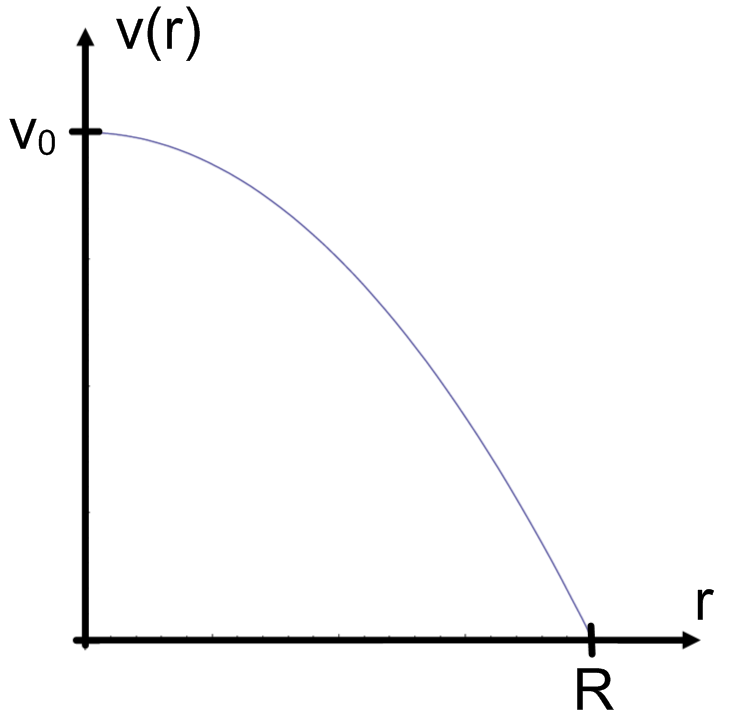
\includegraphics[height=0.4\paperheight]{slike/parabola1.PNG}\qquad{}
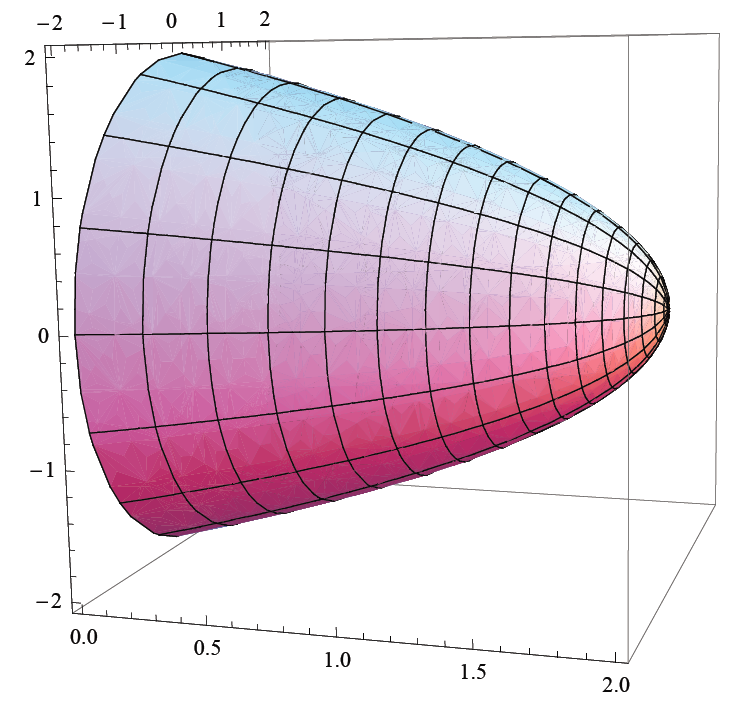
\includegraphics[height=0.4\paperheight]{slike/parabola2.PNG}
\par\end{center}
\begin{alertblock}{Raspodjela brzina kod laminarnog tečenja je parabolična}

\[
v(r)=v_{0}\left(1-\frac{r^{2}}{R^{2}}\right)
\]
\end{alertblock}
\end{frame}

\begin{frame}{Protok kroz cijev}

\begin{itemize}
\item u praksi nas najčešće zanima protok kroz cijev
\item za cijev kružnog presjeka protok je
\[
Q=\intop_{\Omega}vdS=\intop_{\Omega}v(r)rdrd\varphi=\intop_{0}^{2\pi}d\varphi\intop_{0}^{R}v(r)rdr=2\pi\intop_{0}^{R}v(r)rdr
\]
\item pošto znamo $v(r)$ možemo izračunati protok
\item protok je usko vezan sa srednjom brzinom
\[
\bar{v}\equiv\frac{Q}{S}\quad\Rightarrow\quad Q=\bar{v}S
\]
\item dakle, zapravo je svejedno da li računamo protok ili srednju brzinu
\[
\bar{v}=\frac{Q}{S}=\frac{1}{S}\intop_{\Omega}vdS=\frac{2\pi}{\pi R^{2}}\intop_{0}^{R}v(r)rdr=\frac{2}{R^{2}}\intop_{0}^{R}v(r)rdr
\]
\end{itemize}
\end{frame}

\begin{frame}{Srednja brzina kod laminarnog tečenja}

Da bi dobili srednju brzinu kod laminarnog tečenja treba provesti
integraciju za paraboličnu raspodjelu brzina $v(r)=v_{0}\left(1-\frac{r^{2}}{R^{2}}\right)$
\[
\bar{v}=\frac{2}{R^{2}}\intop_{0}^{R}v(r)rdr=\frac{2}{R^{2}}\intop_{0}^{R}v_{0}\left(1-\frac{r^{2}}{R^{2}}\right)rdr=
\]
\[
=\frac{2v_{0}}{R^{2}}\left(\intop_{0}^{R}rdr-\frac{1}{R^{2}}\intop_{0}^{R}r^{3}dr\right)=\frac{2v_{0}}{R^{2}}\left(\frac{R^{2}}{2}-\frac{1}{R^{2}}\frac{R^{4}}{4}\right)=
\]
\[
=2v_{0}\left(\frac{1}{2}-\frac{1}{4}\right)=\frac{v_{0}}{2}
\]

\end{frame}

\begin{frame}{Protok kod laminarnog tečenja: Hagen-Poiseuilleov zakon}

\[
Q=\bar{v}S=\frac{v_{0}}{2}\pi R^{2}=\frac{\pi}{2}\frac{\Delta p}{4\mu L}R^{2}R^{2}=\frac{\pi}{8}\frac{\Delta p}{\mu L}R^{4}
\]

\begin{itemize}
\item u praksi je uobičajeno umjesto polumjera cijevi $R$ koristiti promjer
cijevi $D=2R$
\end{itemize}
\begin{block}{Hagen-Poiseuilleov zakon}

\[
Q=\frac{\pi}{128}\frac{\Delta p}{\mu L}D^{4}
\]
\end{block}
\begin{itemize}
\item protok je proporcionalan razlici tlakova $\Delta p$
\item obrnuto je proporcionalan duljini cijevi $L$ i dinamičkoj viskoznosti
$\mu$
\item ovisi o \alert{četvrtoj potenciji} promjera $D$!
\end{itemize}
\end{frame}

\begin{frame}{Visina gubitaka kod laminarnog tečenja}

\begin{itemize}
\item Hagen-Poiseuilleov zakon možemo okrenuti i pitati kolika je razlika
tlakova $\Delta p$ potrebna da se dobije željeni protok $Q$
\[
Q=\frac{\pi}{128}\frac{\Delta p}{\mu L}D^{4}\quad\Rightarrow\quad\Delta p=\frac{128}{\pi}\frac{\mu L}{D^{4}}Q
\]
\item razlika tlakova zapravo je gubitak specifične energije tekućine zbog
viskoznog trenja
\item gubitke je u praksi uobičajeno iskazivati preko srednje brzine i takozvane\emph{
}\alert{visine gubitaka}
\[
h_{f}=\frac{\Delta p}{\rho g}=\frac{1}{\rho g}\frac{128}{\pi}\frac{\mu L}{D^{4}}\bar{v}\frac{\pi}{4}D^{2}=\frac{32\mu L}{\rho gD^{2}}\bar{v}
\]
\end{itemize}
\begin{alertblock}{}

Kod laminarnog tečenja visina gubitaka $h_{f}$ proporcionalna je
srednjoj brzini $\bar{v}$.
\end{alertblock}
\end{frame}

\section{Turbulentno tečenje}
\begin{frame}{Turbulentno tečenje}

\begin{itemize}
\item tečenje više nije u slojevima --- javljaju se poprečne komponente
brzine koje su okomite na smjer tečenja i miješaju različite slojeve
\item samo tanki, takozvani \alert{rubni sloj} (engl. \emph{boundary layer})
ostaje ``zalijepljen'' za rub cijevi, a ostala tekućina se miješa
i kroz cijeli profil cijevi prolazi praktički istom brzinom koja približno
odgovara srednjoj brzini tečenja $\bar{v}$
\item zbog izuzetno male viskoznosti vode (kinematička viskoznost vode na
$20^\circ C$ je $10^{-6}$ $m^{2}/s$) tečenje vode je najčešće turbulentno
\item prijelaz iz laminarnog u turbulentni režim tečenja vidljiv je u \alert{Reynoldsovom eksperimentu}
\end{itemize}
\end{frame}

\begin{frame}{Reynoldsov broj}

\begin{definition}
Reynoldsov broj
\[
\mathrm{Re}\equiv\frac{\rho\bar{v}D}{\mu}=\frac{\bar{v}D}{\nu}
\]
\end{definition}

Reynoldsov broj je \alert{bezdimenzionalna veličina} i predstavlja
omjer fizikalnih veličina koje su karakteristične za proces tečenja:
\begin{itemize}
\item gustoća $\rho$ i dinamička viskoznost $\mu$ su relevantne karakteristike
tekućine koje utječu na svojstva tečenja
\item $\bar{v}$ je srednja brzina tečenja
\item $D$ predstavlja karakterističnu, tipičnu dimenziju sustava (za slučaj
cijevi kružnog presjeka to je upravo promjer $D$)
\end{itemize}
\end{frame}

\begin{frame}{Interpretacija Reynoldsovog broja}

Provjera da je Reynoldsov broj doista bezdimenzionalna veličina:

\[
[\mathrm{Re}]=\frac{[\rho][\bar{v}][D]}{[\mu]}=\frac{kg\,m^{-3}m\,s^{-1}m}{Pa\,s}=\frac{kg\,m^{-1}s^{-2}}{Nm^{-2}}=\frac{kg\,ms^{-2}}{N}=1
\]

\begin{alertblock}{Reynoldsov broj karakterizira različite režime (modalitete) tečenja:}

\begin{itemize}
\item kad je Re < 2100 tečenje je LAMINARNO
\item kad je Re > 4000 tečenje je TURBULENTNO
\end{itemize}
\end{alertblock}
\begin{itemize}
\item područje vrijednosti Reynoldsovog broja između 2100 i 4000 naziva
se \emph{prijelazno područje} i u njemu se izmjenjuju laminarno i
turbulentno tečenje
\end{itemize}
\end{frame}

\section{Darcy-Weisbachova formula}
\begin{frame}{Visina gubitaka kod turbulentnog tečenja}
\begin{itemize}
\item visinu gubitaka za turbulentno tečenje nije moguće jednostavno izvesti
iz osnovnih principa Newtonove mehanike kao što je to bio slučaj za
laminarno tečenje
\item naravno da se tekućina i dalje giba u skladu sa zakonima klasične
mehanike, ali je zbog miješanja slojeva precizan matematički opis
suviše kompliciran (danas je moguć proračun pomoću računala: \emph{CFD
- Computational Fluid Dynamics})
\item no zbog ogromnog značenja koje tečenje u cijevima ima u praktičnoj
primjeni, kroz povijest su se u inženjerskoj praksi koristile razne
fenomenološke formule (formule izvedene iz praktičnog inženjerskog
iskustva)
\item polovicom 19. stoljeća prevladala je takozvana \alert{Darcy-Weisbachova formula}
\end{itemize}
\end{frame}

\begin{frame}{Darcy-Weisbachova formula}

\begin{block}{Darcy-Weisbachova formula za visinu gubitaka u cijevima}

\[
h_{f}=\lambda\frac{L}{D}\frac{\bar{v}^{2}}{2g}
\]
\end{block}
\begin{description}
\item [{$h_{f}$}] - visina gubitaka ($m$)
\item [{L}] - duljina cijevi ($m$)
\item [{D}] - promjer cijevi ($m$)
\item [{$\bar{v}$}] - srednja brzina ($ms^{-1}$)
\item [{g}] - ubrzanje slobodnog pada ($ms^{-2}$)
\item [{$\lambda$}] - \alert{koeficijent otpora trenja} (bezdimenzionalan)
\end{description}
\end{frame}

\begin{frame}{Koeficijent otpora trenja za laminarno tečenje}

Visinu gubitaka iz Hagen-Poiseuilleovog zakona za laminarno tečenje
u cijevi izjednačimo s Darcy-Weisbachovom formulom
\[
h_{f}=\frac{32\mu L}{\rho gD^{2}}\bar{v}=\lambda\frac{L}{D}\frac{\bar{v}^{2}}{2g}
\]
i riješimo po $\lambda$
\[
\lambda=\frac{32\mu L\bar{v}}{\rho gD^{2}}\frac{D}{L}\frac{2g}{\bar{v}^{2}}=64\frac{\mu}{\rho\bar{v}D}=\frac{64}{\mathrm{Re}}
\]

\begin{block}{}

\begin{itemize}
\item kod laminarnog tečenja koeficijent otpora trenja $\lambda$ ovisi
samo o Reynoldsovom broju
\item relaciju $\lambda=64/\mathrm{Re}$ lako je zapamtiti pa nema potrebe
pamtiti Hagen-Poiseuilleov zakon
\end{itemize}
\end{block}
\end{frame}

\begin{frame}{Koeficijent otpora trenja za turbulentno tečenje}

\begin{itemize}
\item u turbulentnom režimu tečenja koeficijent otpora trenja $\lambda$
ovisi o Reynoldsovom broju i \alert{relativnoj hrapavosti}
\item \alert{apsolutna hrapavost} mjeri se u metrima i označava s $\varepsilon$
\item \alert{relativna hrapavost} definirana je kao omjer apsolutne hrapavosti
i promjera cijevi, dakle $\varepsilon/D$
\item ovisnost $\lambda(\mathrm{Re},\:\varepsilon/D$) je vrlo složena i
određena je eksperimentalnim mjerenjima te se može prikazati u takozvanom
Moodyjevom dijagramu ili parametrizirati različitim formulama od kojih
se najtočnijom smatra Colebrookova formula
\item Colebrookova formula je iterativna pa je za upotrebu praktičnija približna
formula koju su predložili Swamee i Jain
\end{itemize}
\end{frame}

\begin{frame}{Colebrookova i formula Swamee-Jain}

Colebrookova iterativna formula
\[
\frac{1}{\sqrt{\lambda}}=-2,0\log\left(\frac{\varepsilon/D}{3,7}+\frac{2,51}{\mathrm{Re}\sqrt{\lambda}}\right)
\]

\vfill{}

Formula Swamee-Jain
\[
\lambda=\frac{0,25}{\left[\log\left(\frac{\varepsilon/D}{3,7}+\frac{5,74}{\mathrm{Re^{0,9}}}\right)\right]^{2}}
\]

\end{frame}

\begin{frame}{Moodyjev dijagram}

\begin{center}
\vspace{-0.2\paperheight}
\par\end{center}

\begin{center}
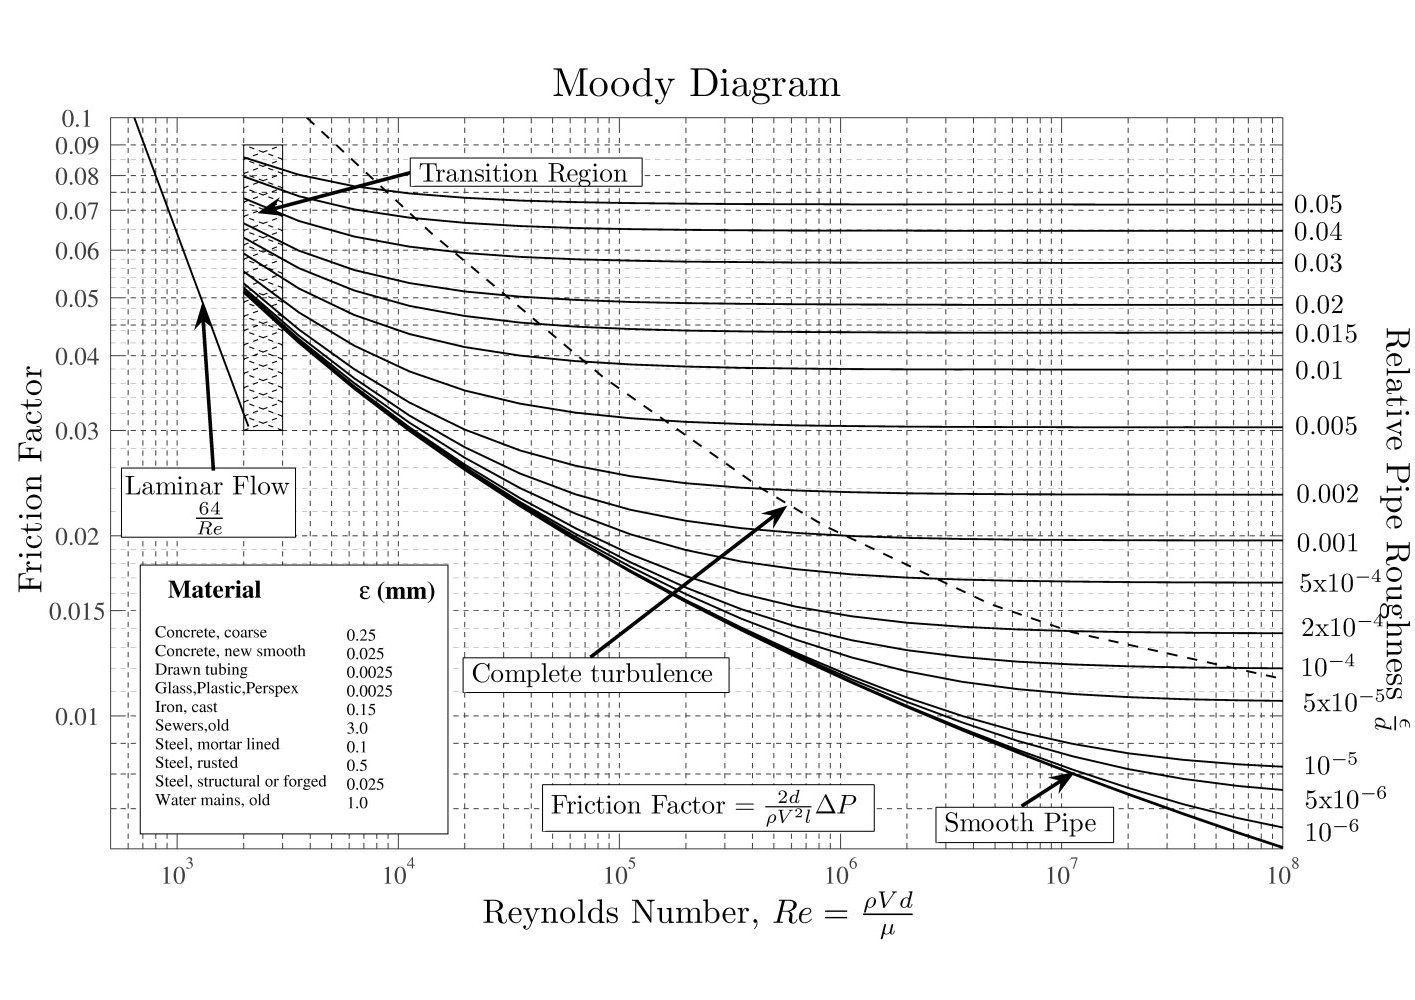
\includegraphics[height=0.76\paperheight]{slike/Moody_diagram}
\par\end{center}

\vspace{-0.1\paperheight}
\textsubscript{{\tiny{}Preuzeto sa \href{https://en.wikipedia.org/wiki/Moody_chart\#/media/File:Moody_diagram.jpg}{https://en.wikipedia.org/wiki/Moody\_chart\#/media/File:Moody\_diagram.jpg}}}
\end{frame}

\end{document}
